\documentclass[11pt]{article}
\usepackage[toc,page]{appendix}
\usepackage{amsmath, amssymb}
\usepackage[utf8]{inputenc}
\usepackage[T1]{fontenc}
\usepackage[style=apa,backend=biber]{biblatex}
%\usepackage{biblatex}
\addbibresource{references.bib}
\usepackage{graphicx}
\usepackage{tikz}
\usetikzlibrary{automata,positioning,shapes.geometric, arrows.meta, fit, backgrounds, calc, chains}
\graphicspath{./images/Easy_Pictures/SMR_MULT_Repackaging}%\usepackage{kpfonts}
\usepackage{float}
\usepackage[margin=1in]{geometry}
\usepackage{cancel}
\usepackage{epsfig}
\usepackage{tikz-3dplot}
\usepackage{darkmode}
\usepackage{dirtytalk}
\usepackage{longtable,booktabs,array}
\usepackage{calc} % for calculating minipage widths
\usepackage[utf8]{inputenc}
\usepackage[T1]{fontenc}
\usepackage{xcolor}
\usepackage{listings}


\usepackage{etoolbox}
\usepackage{hyperref}
\hypersetup{
    colorlinks=true,
    linkcolor=blue,
    filecolor=magenta,      
    urlcolor=cyan,
    pdftitle={Hermeneutic Calculator},
    citecolor=blue,
    }


\urlstyle{same}

\lstdefinestyle{htmlStyle}{
    language=HTML,
    basicstyle=\ttfamily\small,
    keywordstyle=\color{blue}\bfseries,
    commentstyle=\color{gray}\itshape,
    stringstyle=\color{red},
    breaklines=true,
    frame=single,
    numbers=left,
    numberstyle=\tiny\color{gray},
    columns=fullflexible,
}
\lstdefinelanguage{HTML}{
  keywords={<!DOCTYPE, html, head, title, body, h1, h2, h3, p, div, span, a, img, ul, li, table, tr, td, th, style, link, script},
  sensitive=true,
  comment=[l]{//},
  morecomment=[s]{/*}{*/},
  morestring=[b]',
  morestring=[b]"
}
\lstset{style=htmlstyle, language=html}
% Updated to explicitly pass the language option
%\lstinputlisting[style=htmlstyle, language=html]{./html/example.html}
%\usepackage{tocloft}

% Optional: define some custom colors
\definecolor{sliceRed}{RGB}{225,224,91} % matching "varyellow" from your code
\definecolor{linkYellow}{RGB}{255,215,0}  % a golden yellow
\tdplotsetmaincoords{70}{110}

\title{Division Strategies - Dealing by Ones}
\author{Compiled by: Theodore M. Savich}
\date{\today}

\begin{document}
\maketitle

This is a sharing division problem. With sharing division problems, the number of items in each group is unknown, while the number of groups and the total number of items are both known. 

$\fbox{Number of groups} \times \fbox{Unknown Number of items in each group}  = \fbox{Total number of items}$

\subsection*{Transcript}
Video from \textcite{Carpenter1999}. Strategy descriptions and examples adapted from \textcite{HackenbergCourseNotes}. 

\begin{itemize}
    \item \textbf{Teacher:} Mr. Gomez has 12 cupcakes. He wants to put the cupcakes into four boxes, so that there's the same number in each box. How many cupcakes can go in each box?
    \item \textbf{Student:} Okay, 1, 2, 3, 4. I got four boxes, 1, 2, 3, 4, 5, 6, 7, 8, 9, 10, 11,12. Now, one will go in this box, one will go in this box, one will go in this box, one will go in this box. Two will go in this box, two will go in this box, two will go in this box, two will go in this box. Three will go in this box, three will go in this box, three will go in this box, and three, will go in this box. Three cupcakes can go in each box. 
    \item \textbf{Teacher:} Nice. Thank you, Alex.
\end{itemize}

Alex began by placing 4 unifix cubes of the same color on the table, each one standing in for a different box. He then selected 12 additional cubes to represent 12 cupcakes. One by one, he distributed a cube from this pile to each box, repeating the process until he had used all the cupcake cubes. When he finished, he observed that each box contained 3 cubes, so the answer is 3 cupcakes per box.


\subsection*{Dealing by Ones}

\subsubsection*{Strategy Overview}
\textbf{Dealing by Ones} is a foundational division strategy where the division is performed by incrementally removing one item at a time and counting the number of groups formed. This method is particularly useful for simple division problems and serves as the basis for more advanced strategies.

\subsubsection*{Automaton Design}
We design a \textbf{Pushdown Automaton (PDA)} that systematically removes one element from the total and increments the group count until all elements have been distributed.

\subsubsection*{Automaton Tuple}
The PDA is defined as the 7-tuple
\[
M = (Q,\, \Sigma,\, \Gamma,\, \delta,\, q_{0/accept},\, \#,\, F)
\]
where:
\begin{itemize}
    \item \(Q = \{q_{0/accept},\, q_{\text{remove}},\, q_{\text{output}}\}\) is the set of states. Here, \(q_{0/accept}\) is the merged start and accepting state.
    \item \(\Sigma = \{E\}\) is the input alphabet, where \(E\) represents an element.
    \item \(\Gamma = \{\#, G, E\}\) is the stack alphabet:
    \begin{itemize}
        \item \(\#\) is the bottom-of-stack marker.
        \item \(G\) represents a group identifier.
        \item \(E\) represents an element.
    \end{itemize}
    \item \(q_{0/accept}\) is the start (and accepting) state.
    \item \(\#\) is the initial stack symbol.
    \item \(F = \{q_{0/accept}\}\) is the set of accepting states.
\end{itemize}

\subsubsection*{Transition Function}
The key transitions of the PDA are as follows:
\begin{enumerate}
    \item \textbf{Initialization:}  
    \[
    \delta(q_{0/accept},\, \varepsilon,\, \varepsilon) = (q_{\text{remove}},\, \#)
    \]
    (Push the bottom marker \(\#\) and move to the removal phase.)
    
    \item \textbf{Removing Elements:}  
    \[
    \delta(q_{\text{remove}},\, \varepsilon,\, E) = (q_{\text{remove}},\, \varepsilon \text{ (pop } E\text{)}\; \text{followed by pushing } G)
    \]
    (For each \(E\) encountered on the stack, pop it and push \(G\) to record one completed group.)
    
    \item \textbf{Transition when no \(E\) remains:}  
    \[
    \delta(q_{\text{remove}},\, \varepsilon,\, \#) = (q_{\text{output}},\, \#)
    \]
    (When no \(E\) is left (only the bottom marker remains), move to the output phase.)
    
    \item \textbf{Outputting the Result:}  
    \[
    \delta(q_{\text{output}},\, \varepsilon,\, x) = (q_{0/accept},\, x)
    \]
    (Count the number of \(G\) symbols to determine the quotient; output the final count and return to the merged start/accept state.)
\end{enumerate}

\subsubsection*{State Transition Table}
\begin{center}
\begin{tabular}{|c|c|c|c|c|c|}
\hline
\textbf{Current} & \textbf{Input} & \textbf{Stack } & \textbf{Next} & \textbf{Stack} &\textbf{Description}\\
\textbf{State} &  \textbf{Symbol} & \textbf{Top} & \textbf{State} & \textbf{Operation} &\\
\hline
\(q_{0/accept}\) & \(\varepsilon\) & --- & \(q_{\text{remove}}\) & Push \(\#\) & Initialization \\
\hline
\(q_{\text{remove}}\) & \(\varepsilon\) & \(E\) & \(q_{\text{remove}}\) & Pop \(E\), push \(G\) & Remove one element, \\
& & & & & increment group count \\
\hline
\(q_{\text{remove}}\) & \(\varepsilon\) & \(\#\) & \(q_{\text{output}}\) & No change & All \(E\)'s removed \\
\hline
\(q_{\text{output}}\) & \(\varepsilon\) & (Any) & \(q_{0/accept}\) & Output final count & Output quotient \\
& & & & & (number of \(G\)'s) \\
\hline
\end{tabular}
\end{center}

\subsubsection*{Circular PDA Diagram}
\begin{center}
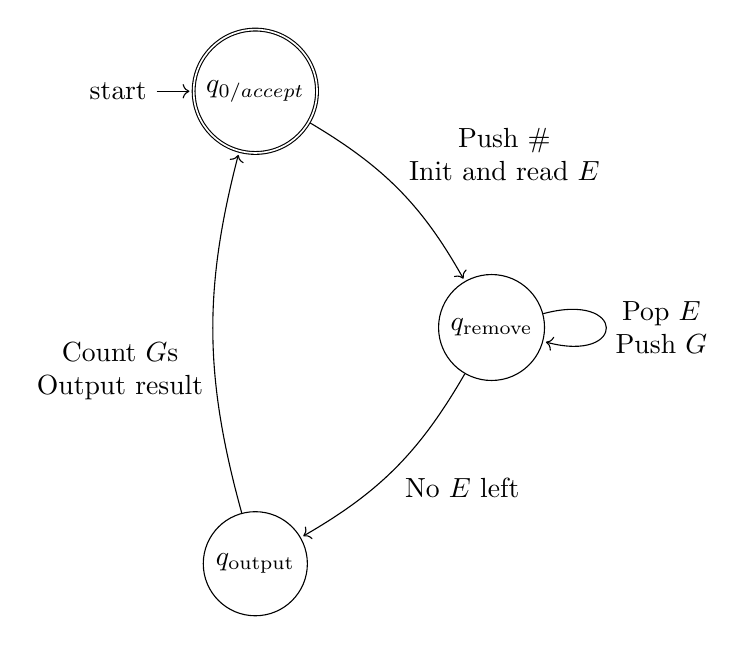
\begin{tikzpicture}[
    shorten >=1pt,
    auto,
    node distance=3cm,
    every state/.style={minimum size=1cm}
]
    % Arrange 3 states on a circle:
    % q_{0/accept} at 90°, q_remove at 0°, q_output at 270°.
    \node[state, initial, accepting] (q0) at (90:3cm) {$q_{0/accept}$};
    \node[state] (q1) at (0:3cm) {$q_{\text{remove}}$};
    \node[state] (q2) at (270:3cm) {$q_{\text{output}}$};
    
    \path[->]
        (q0) edge[bend left=15] node[above right, align=center] {Push \(\#\)\\Init and read \(E\)} (q1)
        (q1) edge[loop right] node[right, align=center] {Pop \(E\) \\Push \(G\)} (q1)
        (q1) edge[bend left=15] node[below right, align=center] {No \(E\) left} (q2)
        (q2) edge[bend left=15] node[below left, align=center] {Count \(G\)s\\Output result} (q0);
\end{tikzpicture}
\end{center}

\subsubsection*{Example Execution}
\textbf{Problem:} Divide 7 items into groups of 1.

\begin{enumerate}
    \item \textbf{Start:}  
    \begin{itemize}
        \item Initial Stack: \(\#\, E\, E\, E\, E\, E\, E\, E\) (7 \(E\)'s representing 7 items).
    \end{itemize}
    \item \textbf{Removing Elements:}
    \begin{itemize}
        \item For each \(E\) popped, a \(G\) is pushed. After 7 removals, the stack becomes: \(\#\, G\, G\, G\, G\, G\, G\, G\).
    \end{itemize}
    \item \textbf{Outputting the Result:}
    \begin{itemize}
        \item The automaton counts the 7 \(G\)'s and outputs the result (7 groups of 1).
    \end{itemize}
\end{enumerate}

\subsubsection*{HTML Implementation}
\lstinputlisting[style=htmlStyle, language=html]{./new_html/SMR_DIV_Dealing_By_Ones.html}

\printbibliography
\end{document}